%
% teil1.tex -- Beispiel-File für das Paper
%
% (c) 2020 Prof Dr Andreas Müller, Hochschule Rapperswil
%
% !TEX root = ../../buch.tex
% !TEX encoding = UTF-8
%
\section{Stochastische Differenzialgleichungen\label{brown:SDGL}}
\rhead{Stochastische DGLs}

Ist einer gewöhnlichen Differenzialgleichtung (DGL) gegeben, kann das Verhalten eines Systems unter Berücksichtigung der Anfangsbedingungen vorhergesagt werden. Vom Anfangswert aus entwickelt sich die Funktion gemäss der Startbedingung und dem durch die DGL gegebenen Vektorfeld. Für einen bestimmten Startwert und wert der Laufvariabel, kann ein bestimmter Funktionswert ermittelt werden.

In vielen Bereichen entspricht ein solch deterministisches System  nicht der Realität und suggeriert eine Aussagekraft, welche sich nicht mit der Wirklichkeit deckt und somit einen eher Geringen Wert hat. In gewissen Systemen können kleine Störeinflüsse das Resultat maßgeblich beeinflussen. Dies führt dazu, dass sich die Lösung einer DGL  gegenüber der Realität, zum Beispiel durch Rauschen, nicht perfekt deckt oder sogar komplett divergiert.

Ein gutes Beispiel dafür ist folgendes System:
\begin{equation}
	\frac{dy}{dt} = x - y
\end{equation}

\begin{figure}
	\centering
	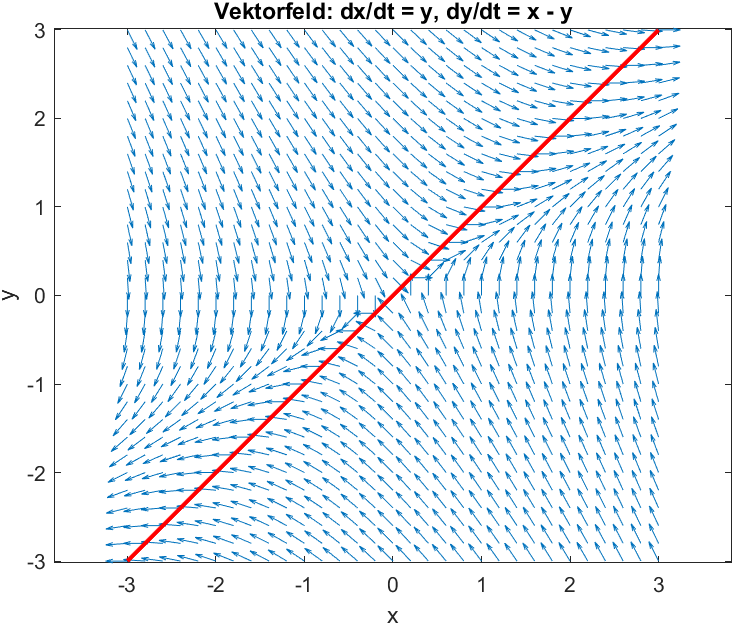
\includegraphics[width=\linewidth]{papers/brown/images/vektorfeld_01.png}
	\caption{My caption}
\end{figure}

In diesem System konvergieren alle Trajektorien zum Ursprung, ausser diese, welche Ihren Startwert auf der Geraden $ y = x $ haben. Also kann ein kleiner Störeinfluss darüber entscheiden ob, der Wert zum gegen (0,0) konvergiert oder nach Unendlich divergiert. Wobei bei diesem Beispiel gesagt werden muss, dass in Realität der Startwert nie exakt auf die Gerade $ y = x $ fallen würde.




Um diesem Umstand gerecht zu werden, kann man die Möglichkeit von Zufälligen Störungen beim Aufstellen des Modells miteinbeziehen - et. voilà, man hat eine stochastische Differenzialgleichung (SDE).

Nun ist die Aussage, also die Lösung der SDE, nicht mehr ein Zustand zum Zeitpunkt $ t $, sondern eine Wahrscheinlichkeitsverteilung über die verschiedenen möglichen Endzustände unter Einbezug von zufälligen Störungen.

Formal kann dies folgendermaßen notiert werden, 

\begin{equation}
\label{brown:SDGL:whiteNoise}
\dot{X}(t) = b(X(t)) + B(X(t))\xi(t) \quad (t>0)
\end{equation}

wobei B eine n x m Matrize mit Faktoren ist, welche beschreiben, wie sich Störungen auf die unterschiedlichen ..... des Systems auswirken. $ m $ ist die Dimension der Störfunktion. Also $ m $ eindimensionales "white noise".

\begin{align*}
		b = 
	\begin{pmatrix}
		b_{1} \\
		...\\
		b_{m}\\ 
	\end{pmatrix}
	, \quad
	B = 
	\begin{pmatrix}
		B_{11} & ... & B_{1m} \\
		& ... & \\
		B_{n1} & ... & B_{nm} 
	\end{pmatrix}
\end{align*}


\subsection{Rauschen als Random Walk und Wiener Prozess
\label{brown:SDGL:Wiener}}

Um das sogenannte \textit{white noise} zu modellieren, muss eine Definition für einen stochastischen Prozess gefunden werden. Zwei zentrale Konzepte sind der \textit{random walk} und der Wienerprozess.

\textbf{Random Walk:}
Bei einem Random Walk beginnt man an einem Ausgangspunkt (normalerweise 0) und macht bei jedem Zeitschritt eine zufällige Schritt nach vorne oder hinten, oft dient dazu die Beinominalverteilung, wobei auch asymmetrische Verteilungen verwendet werden können. Die Schrittlänge und Richtung kann ebenfalls durch eine unabhängige Wahrscheinlichkeitsverteilung bestimmt werden order als konstant definiert sein.

\textbf{Wiener-Prozess:}
Der Wiener-Prozess ist ein kontinuierlicher stochastischer Prozess, er kann als Grenzwert eines Random Walks betrachtet werden, wenn die Zeitschritte gegen null gehen und die Schrittlängen normalverteilt sind. Speziell dabei ist, dass unabhängig von der verstrichenen Zeit der Erwartungswert der Startpunkt bleibt.

Man könnte also den Random Walk als eine diskrete Version eines Wiener-Prozesses bezeichnen oder umgekehrt, dass ein Wiener-Prozess eine kontinuierliche Version eines Random Walks ist. Sie unterscheiden sich jedoch bezüglich ihrer zeitlichen Diskretisierung und in den verwendeten Wahrscheinlichkeitsverteilungen.

Für die Modellierung von stochastischem Verhalten, ist der Wiener Prozess $ W(t) $ ein zentrales Konzept, welches folgendermaßen definiert ist:
\begin{itemize}
	\item $ W(0) = 0 $; Der Startwert von $ t = 0 $ ist 0.
	\item $ W(t_{1}) - W(t_{2}) $ ist ein normalverteilte Zufalls-Variable mit Erwartungswert 0 und Varianz $ t_{1} - t_{2} $.
	\item Zu jedem weiteren Zeitpunkt $ t_{n} $ ist die Zufalls-Variable unabhängig von allen vorhergehenden Werten.
\end{itemize}

Weiter wird auf den Wienerprozess nicht eingegangen, da dieser ausführlich im Kapitel \glqq \textit{8.1 Modell für Rauschen: der Wiener-Prozess}\glqq{} des Buches vom Mathematischen Seminar über Differenzialgleichungen beschrieben wird.

\textit{White noise} $ \xi(t) $ kann als die Ableitung vom Wienerprozess $ \frac{dW(t)}{dt} $ modelliert werden. Somit kann die SDGL aus \ref{brown:SDGL:whiteNoise} folgendermaßen geschrieben werden:

\begin{equation}
	\frac{dX(t)}{dt} = b(X(t)) + B(X(t)) \frac{dW(t)}{dt} \quad (t>0)
\end{equation}

Nun sollte man mit $ dt $  multiplizieren, da die Gleichung so nicht sinnvoll ist, denn $ \frac{dW(t)}{dt} $ ist nicht differenzierbar. Dies ist den Eigenschaften des Wienerprozesses geschuldet. Gemäß der Definition ändert sich die Zufalls variable in jedem Schritt dem Erwartungswert und der Varianz entsprechend, ohne dabei von vorhergehenden Werten abzuhängen. Dieses unstetige verhalten ist nicht auf Grund (nicht definierter) Änderungsraten nicht differenzierbar.
! Überarbeiten, nicht differenzierbar? ! 

Bei SDGLs wird das $ dt $ im Nenner oft mit $ dt $ multipliziert, um die Gleichung in die sogenannte \glqq{}Ito-Form\glqq{} zu bringen, welche leichter zu interpretieren und zu bearbeiten ist.

\begin{equation}
	dX(t) = b(X(t)) dt + B(X(t)) dW(t)
\end{equation}

%In dieser Form erkennt man auch besser, dass die SDGL aus zwei Teilen besteht. Der Term $ b((X(t)) $ ist der \glqq{}Drift\glqq{}-Term, der den deterministischen Teil der Bewegung darstellt, während $ B((X(t)) $ der \glqq{}Diffusions- oder Volatilitäts-Term\glqq{} ist, der den stochastischen Teil der Bewegung darstellt.

% So kommt man auf die ITO-sche Kettenregel????

Man kann dem Wiener Prozess auch fraktale Eigenschaften zusprechen, da man den Ausschnitt des zufällig beeinflussten Prozesses beliebig gross oder klein wählen kann und die keinen Einfluss auf die Eigenschaften des beobachteten Verhalten hat.


\subsection{Simulation mittels der Euler-Maruyama-Methode
\label{brown:Simulation}}
\rhead{Simulation} %Kurz-Titel der Section

Die Brownsche Bewegung kann relativ einfach simuliert werden mittels der Eueler-Maruyama-Methode.

Die Euler-Maruyama-Methode ist eine numerische Methode zur Simulation von stochastischen Differentialgleichungen (SDE). SDEs sind Differenzialgleichungen, welche den Einfluss von zufälligen Prozessen, wie zum Beispiel Rauschen, auf ein dynamisches System berücksichtigen können. Sie bestehen aus einem deterministischen Anteil, der die zugrundeliegende Dynamik beschreibt, und einem stochastischen Anteil, der einen zufälligen Einfluss in Betracht zieht. Die Methode basiert auf der bekannten Euler-Methode zur Lösung von gewöhnlichen Differentialgleichungen (ODEs). Die Idee ist, die SDE in diskrete Zeitschritte zu zerlegen und den deterministischen und stochastischen Anteil separat zu behandeln. Die Methode hat zwar gewisse Einschränkungen hinsichtlich ihrer Genauigkeit und Stabilität, ist aber dennoch mitunter auf Grund ihrer Einfachheit weit verbreitet.

Gegeben sei eine SDE der folgenden Form:
\begin{equation}
	\mathrm{d}X(t) = a(X(t), t) \mathrm{d}t + b(X(t), t) \mathrm{d}W(t),
\end{equation}
wobei $ a(X(t), t) $ den deterministische Anteil darstellt, $ b(X(t), t) $ der stochastische Anteil ist und $ W(t) $ ein Wiener-Prozess ist, der das Rauschen repräsentiert. Die Methode beginnt mit einer Anfangsbedingung $X(0) = X_0$.

Um die SDE mit der Euler-Maruyama-Methode zu simulieren, geht man wie folgt vor:

\begin{enumerate}
	\item Man wählt eine Schrittweite $\Delta t > 0$ und teilt das Zeitintervall $[0, T]$ in $N$ gleich große Teilintervalle der Länge $\Delta t$: $t_0 = 0, t_1 = \Delta t, \dots, t_i = i\Delta t, \dots, t_N = T$.
	\item Für jeden Zeitschritt $i$ von $0$ bis $N-1$ werden die Werte der Funktion $X(t)$ an den diskreten Zeitpunkten $t_i$ berechnet,
	\begin{equation}
		X(t_{i+1}) = X(t_i) + a(X(t_i), t_i) \Delta t + b(X(t_i), t_i) \sqrt{\Delta t} \cdot Z_i,
	\end{equation}
	wobei $Z_i$ unabhängige standardnormalverteilte Zufallsvariablen sind.
	\item Diese Berechnungen führt man iterativ für alle Zeitschritte durch.
\end{enumerate}

\begin{equation}
	X_{n+1} = X_n + f(X_n,t_n) \Delta t + g(X_n,t_n) \Delta W_n
\end{equation}

Diese Funktion $ f(X_n,t_n) $ beschreibt dabei den deterministischen Teil der SDE, im Kontext der Brown'schen Bewegung kann man es auch "drift nennen", welcher nicht nur von zufälligen Einflüssen bestimmt ist. Dies ist auch der Teil, der durch eine harmonische Analyse untersucht werden kann. Das Rauschen ("white noise"), welches hier mit $ g(X_n,t_n) $ beschrieben ist, enthält keine Information und kann somit nicht analysiert werden. $ \Delta W $ beschreibt die Geschwindigkeit, mit welcher der stochastische Prozess ablaufen soll und $ W_n $  beschreibt den Wiener Prozess oder die Brownische Bewegung als Ganzes.

\begin{figure}
	\centering
	\begin{minipage}{0.45\textwidth}
		\centering
		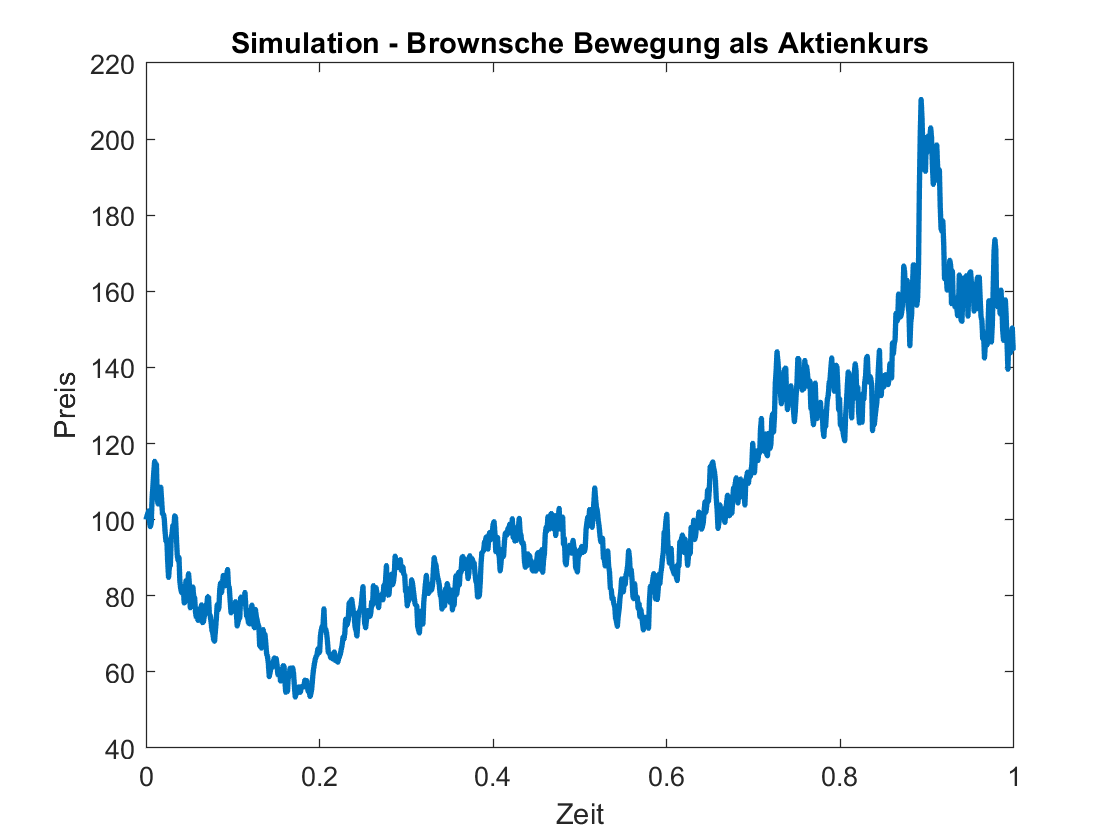
\includegraphics[width=\linewidth]{papers/brown/images/Aktienkurs-als-Brownische-Bewegung_2.png}
		\caption{1D Brownische Bewegung als Aktienkurs}
	\end{minipage}
	\hspace{0.05\linewidth}
	\begin{minipage}{0.45\textwidth}
		\centering
		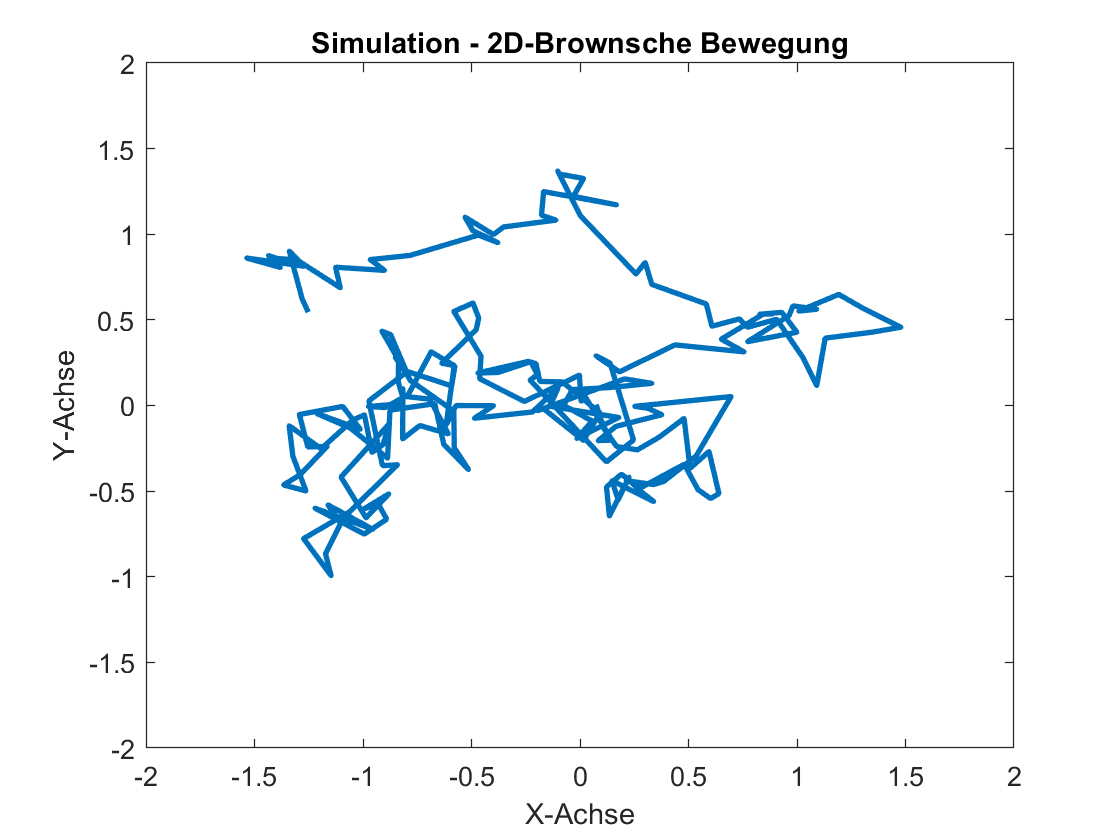
\includegraphics[width=\linewidth]{papers/brown/images/Brownische-Bewegung-Simuliert_2.png}
		\caption{Simulation einer Brownischen Bewegung in 2D}
	\end{minipage}
\end{figure}

In der Abbildung ... ist wurde diese Simulations-Methode in einer Dimension angewandt. Man kann vielleicht schon erahnen, dass die zugrundeliegende Mathematik auf Börsenkurse anwendbar sein könnte. Führt man die Simulation für zwei Achsen durch und verbindet die einzelnen Simulationsschritte mit Linien, ergibt sich das Bild einer typischen Brownischen Bewegung.


\subsection{ITO
\label{brown:ito}}
\rhead{Ito} %Kurz-Titel der Section
Itō Kiyoshi war ein japanischer Mathematiker, der seine Kariere der Stochastik widmete und heute als Begründer der stochastischen Analysis zählt. So legte er auch einen Grossteil des Fundaments auf dem stochastische Differenzialgleichungen beruhen.

Ein wichtiges Werkzeug, um mit stochastischen DIfferenzialgleichungen umzugenhen ist das Äquivalent zur Kettenregel und der Substitutionsregel, dem sogenannten Lemma von Ito. Dieses wird auch im Abschnitt XXXX für das Black-Scholes-Merton Modell verwendet. Auch nach ihm benannt ist die "ito-Form", in welcher die Gleichungen notiert sind XXX.

Hier ein Beispiel:

Die stochastische Differentialgleichung (SDG) für einen Prozess X(t):
\begin{equation}
	dX = a(X,t) dt + b(X,t) dW
\end{equation}

Angenommen, wir haben eine Funktion f(X,t), wobei X eine Lösung der obigen SDG ist. Dann kann die Änderung von f in Bezug auf X und t wie folgt geschrieben werden:

Die Funktion f(X,t) und das Ito-Lemma:
\begin{equation}
	df = \frac{\partial f}{\partial t} dt + \frac{\partial f}{\partial X} dX + \frac{1}{2} \frac{\partial^2 f}{\partial X^2} (dX)^2	
\end{equation}

%Dabei sind ∂f/∂t und ∂f/∂X die partiellen Ableitungen von f nach t und X, und ∂²f/∂X² ist die zweite partielle Ableitung von f nach X. Der Term (dX)² ist im Ito-Kalkül durch (b^2 dt) ersetzt, was auf die Eigenschaften der Brown'schen Bewegung (oder Wiener-Prozess) zurückzuführen ist.

Dieses Lemma erlaubt es uns, Differentialgleichungen für Funktionen von stochastischen Prozessen abzuleiten, was bei der Lösung von SDGs hilfreich ist.

Das Einsetzen der SDG in das Ito-Lemma ergibt:
\begin{equation}
	df = \frac{\partial f}{\partial t} dt + \frac{\partial f}{\partial X} (a dt + b dW) + \frac{1}{2} \frac{\partial^2 f}{\partial X^2} (b^2 dt)
\end{equation}

Die Funktion $ a(X,t) $ ist der "Drift"-Term, der den deterministischen Teil der Bewegung darstellt, während $ b(X,t) $ der "Diffusion"- oder "Volatilitäts"-Term ist, der den stochastischen Teil der Bewegung darstellt.

Ein wichtiger Aspekt des Ito-Kalküls ist die Ito'sche Lemma, eine Erweiterung der Kettenregel aus der gewöhnlichen Differentialrechnung für Funktionen von stochastischen Prozessen. Die genaue Form des Ito'schen Lemmas kann komplex sein, aber in einer einfacheren Form lautet es wie folgt:


